\chapter{Resultados e Discussão}
\label{cap:resultados}

Este capítulo apresenta os resultados obtidos sobre o conjunto de teste (2024 a 2026, 137 mesorregiões, 16.988 mesorregião-semanas) e os discute à luz da pergunta de pesquisa. A Seção~\ref{sec:res_dados} descreve a base de modelagem e o efeito das correções de dados. As Seções~\ref{sec:res_baselines} e~\ref{sec:res_2024} comparam o XGBoost com os previsores ingênuos, no agregado e ano a ano. As Seções~\ref{sec:res_clima} a~\ref{sec:res_shap} tratam da contribuição do clima. A Seção~\ref{sec:res_risco} avalia a classificação de risco, a Seção~\ref{sec:res_df} apresenta o recorte do Distrito Federal e a Seção~\ref{sec:res_complementar} confronta os achados com o experimento complementar.

\section{Base de Modelagem e Efeito das Correções de Dados}
\label{sec:res_dados}

A base final reúne 60.554 mesorregião-semanas, de 2018 a 2026, com cobertura climática de 90,1\%. A cobertura variou entre os anos (Figura~\ref{fig:cobertura_inmet}): foi máxima em 2018 e 2019 (97,4\% e 97,8\%) e mínima em 2021 (81,3\%) e em 2026 (80,0\%, ano ainda incompleto). A queda em 2021 coincide com o aumento das semanas de baixa cobertura das estações automáticas nesse ano. Como o XGBoost trata valores ausentes nativamente, as semanas sem clima foram mantidas, e a comparação entre os modelos com e sem clima é feita sobre as mesmas linhas.

\begin{figure}[htb]
    \centering
    \caption{Proporção de mesorregião-semanas com dados climáticos, por ano}
    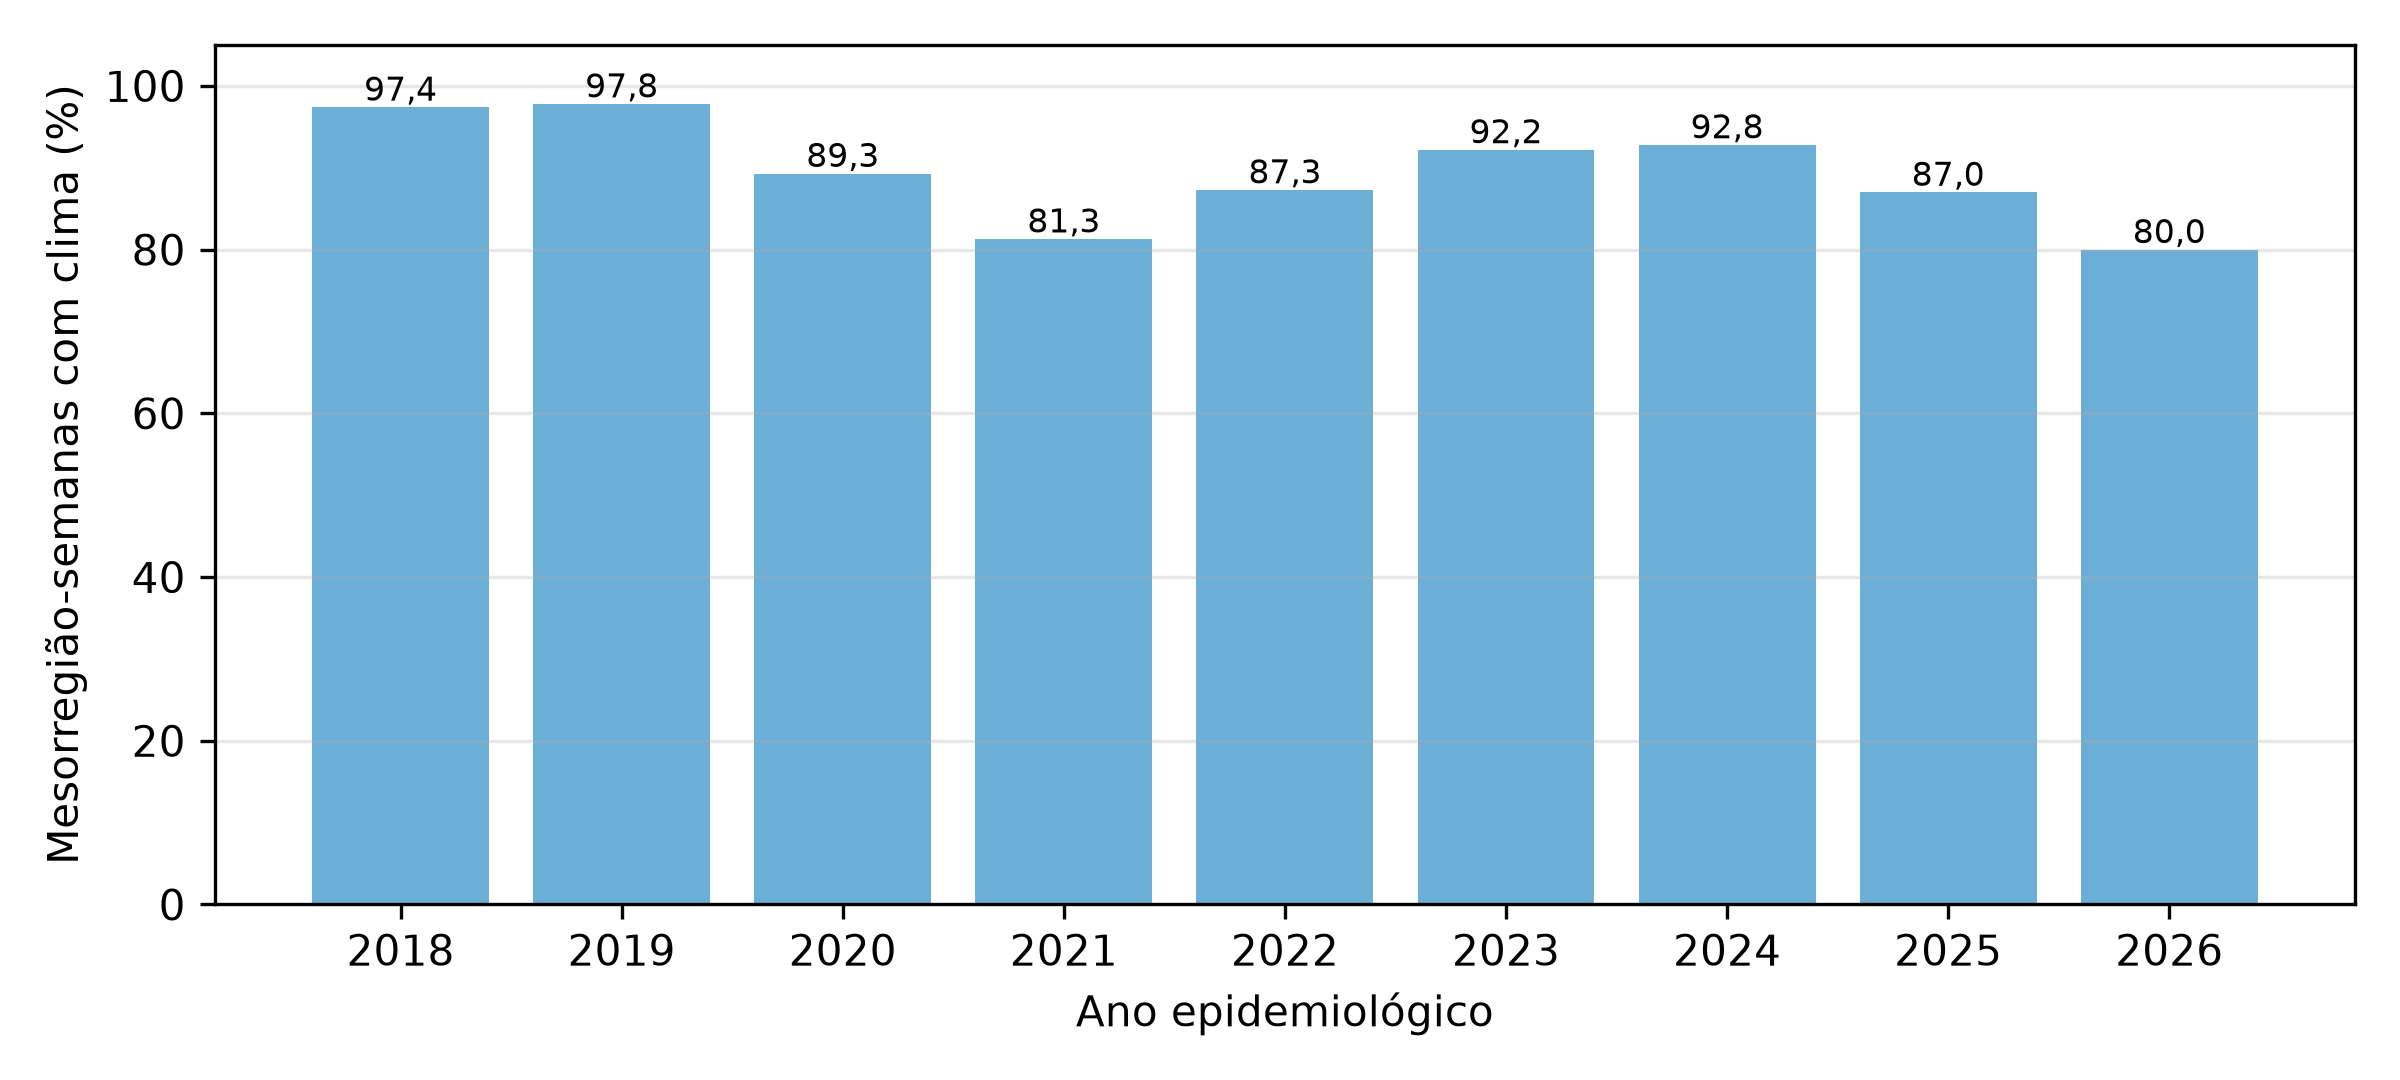
\includegraphics[width=0.8\textwidth]{figuras/resultados/fig_cobertura_inmet_ano.png}
    \label{fig:cobertura_inmet}
    \fonte{Elaboração própria a partir de \citeonline{inmet2025}.}
\end{figure}

A Tabela~\ref{tab:antes_depois} compara a mesma pipeline executada antes e depois das correções descritas na Seção~\ref{sec:correcoes}, com o mesmo conjunto de teste. As correções melhoraram o desempenho de todas as variantes, e duas conclusões se inverteram. Primeiro, o clima passou a ajudar de forma significativa nos cenários de atraso na notificação, nos quais antes a diferença era negativa e não significativa. Segundo, a variável climática mais associada aos casos deixou de ser a ``umidade'', cujo limiar de 15,7\% era, na verdade, uma temperatura de ponto de orvalho em graus Celsius, e passou a ser a temperatura mínima, com limiar fisicamente plausível.

\begin{table}[htb]
\centering
\caption{Resultados da pipeline mesorregional antes e depois das correções de dados}
\label{tab:antes_depois}
\small
\begin{tabular}{|p{0.44\textwidth}|c|c|}
\hline
\textbf{Indicador} & \textbf{Antes} & \textbf{Depois} \\ \hline
$R^2_{\log}$ do modelo A (só SINAN) & 0,843 & 0,859 \\ \hline
$R^2_{\log}$ do modelo C (SINAN + INMET enriquecido) & 0,853 & 0,870 \\ \hline
Ganho do clima com atraso de 4 semanas ($\Delta R^2_{\log}$) & $-$0,0006 ($p=0{,}60$) & +0,0047 ($p<0{,}001$) \\ \hline
Ganho do clima com atraso de 8 semanas ($\Delta R^2_{\log}$) & $-$0,0013 ($p=0{,}22$) & +0,0035 ($p<0{,}001$) \\ \hline
\textit{Walk-forward}: janelas em que C supera A & 3 de 5 & 4 de 4 \\ \hline
Melhor variável climática no SHAP (posição) & pressão (12.ª) & temp. mínima (20.ª) \\ \hline
Limiar climático de destaque & ``umidade'' 15,7 & temp. mínima 13,8~$^\circ$C \\ \hline
\end{tabular}
\fonte{Elaboração própria. Antes: relatórios do PR \#1 do repositório MODELO-PREVISAO; depois: pipeline reprocessada.}
\end{table}

No experimento complementar, a correção do vazamento no rótulo de risco mostrou a dimensão desse viés: com os limiares calculados sobre toda a série, o F1 macro aparecia inflado entre 0,004 e 0,107 e a AUC entre 0,001 e 0,074, conforme o nível de agregação.

\section{Comparação com os Previsores de Referência}
\label{sec:res_baselines}

A Tabela~\ref{tab:baselines} e a Figura~\ref{fig:baselines} apresentam o principal resultado do trabalho. Na escala logarítmica, as três variantes do XGBoost superam todos os baselines: o modelo C alcança $R^2_{\log}=0{,}870$, contra 0,808 da persistência. O MAE também favorece o modelo (252 contra 277 notificações por mesorregião-semana). Na escala original, porém, a ordem se inverte: a persistência obtém $R^2=0{,}668$, praticamente o dobro do modelo C (0,344), e um RMSE 29\% menor.

\begin{table}[htb]
\centering
\caption{Desempenho no conjunto de teste (2024 a 2026)}
\label{tab:baselines}
\small
\begin{tabular}{|l|c|c|r|r|}
\hline
\textbf{Modelo} & \textbf{$R^2_{\log}$} & \textbf{$R^2$} & \textbf{MAE} & \textbf{RMSE} \\ \hline
Persistência & 0,808 & \textbf{0,668} & 277,1 & \textbf{1.495,6} \\ \hline
Média móvel (4 semanas) & 0,757 & 0,459 & 361,9 & 1.909,6 \\ \hline
Sazonal (ano anterior) & 0,356 & $-$0,719 & 712,9 & 3.404,9 \\ \hline
XGBoost A (só SINAN) & 0,859 & 0,280 & 271,7 & 2.203,7 \\ \hline
XGBoost B (+ INMET bruto) & 0,868 & 0,333 & 252,6 & 2.121,3 \\ \hline
XGBoost C (+ INMET enriquecido) & \textbf{0,870} & 0,344 & \textbf{252,2} & 2.103,2 \\ \hline
\end{tabular}
\fonte{Elaboração própria.}
\end{table}

\begin{figure}[htb]
    \centering
    \caption{$R^2$ nas escalas logarítmica e original: XGBoost e previsores ingênuos}
    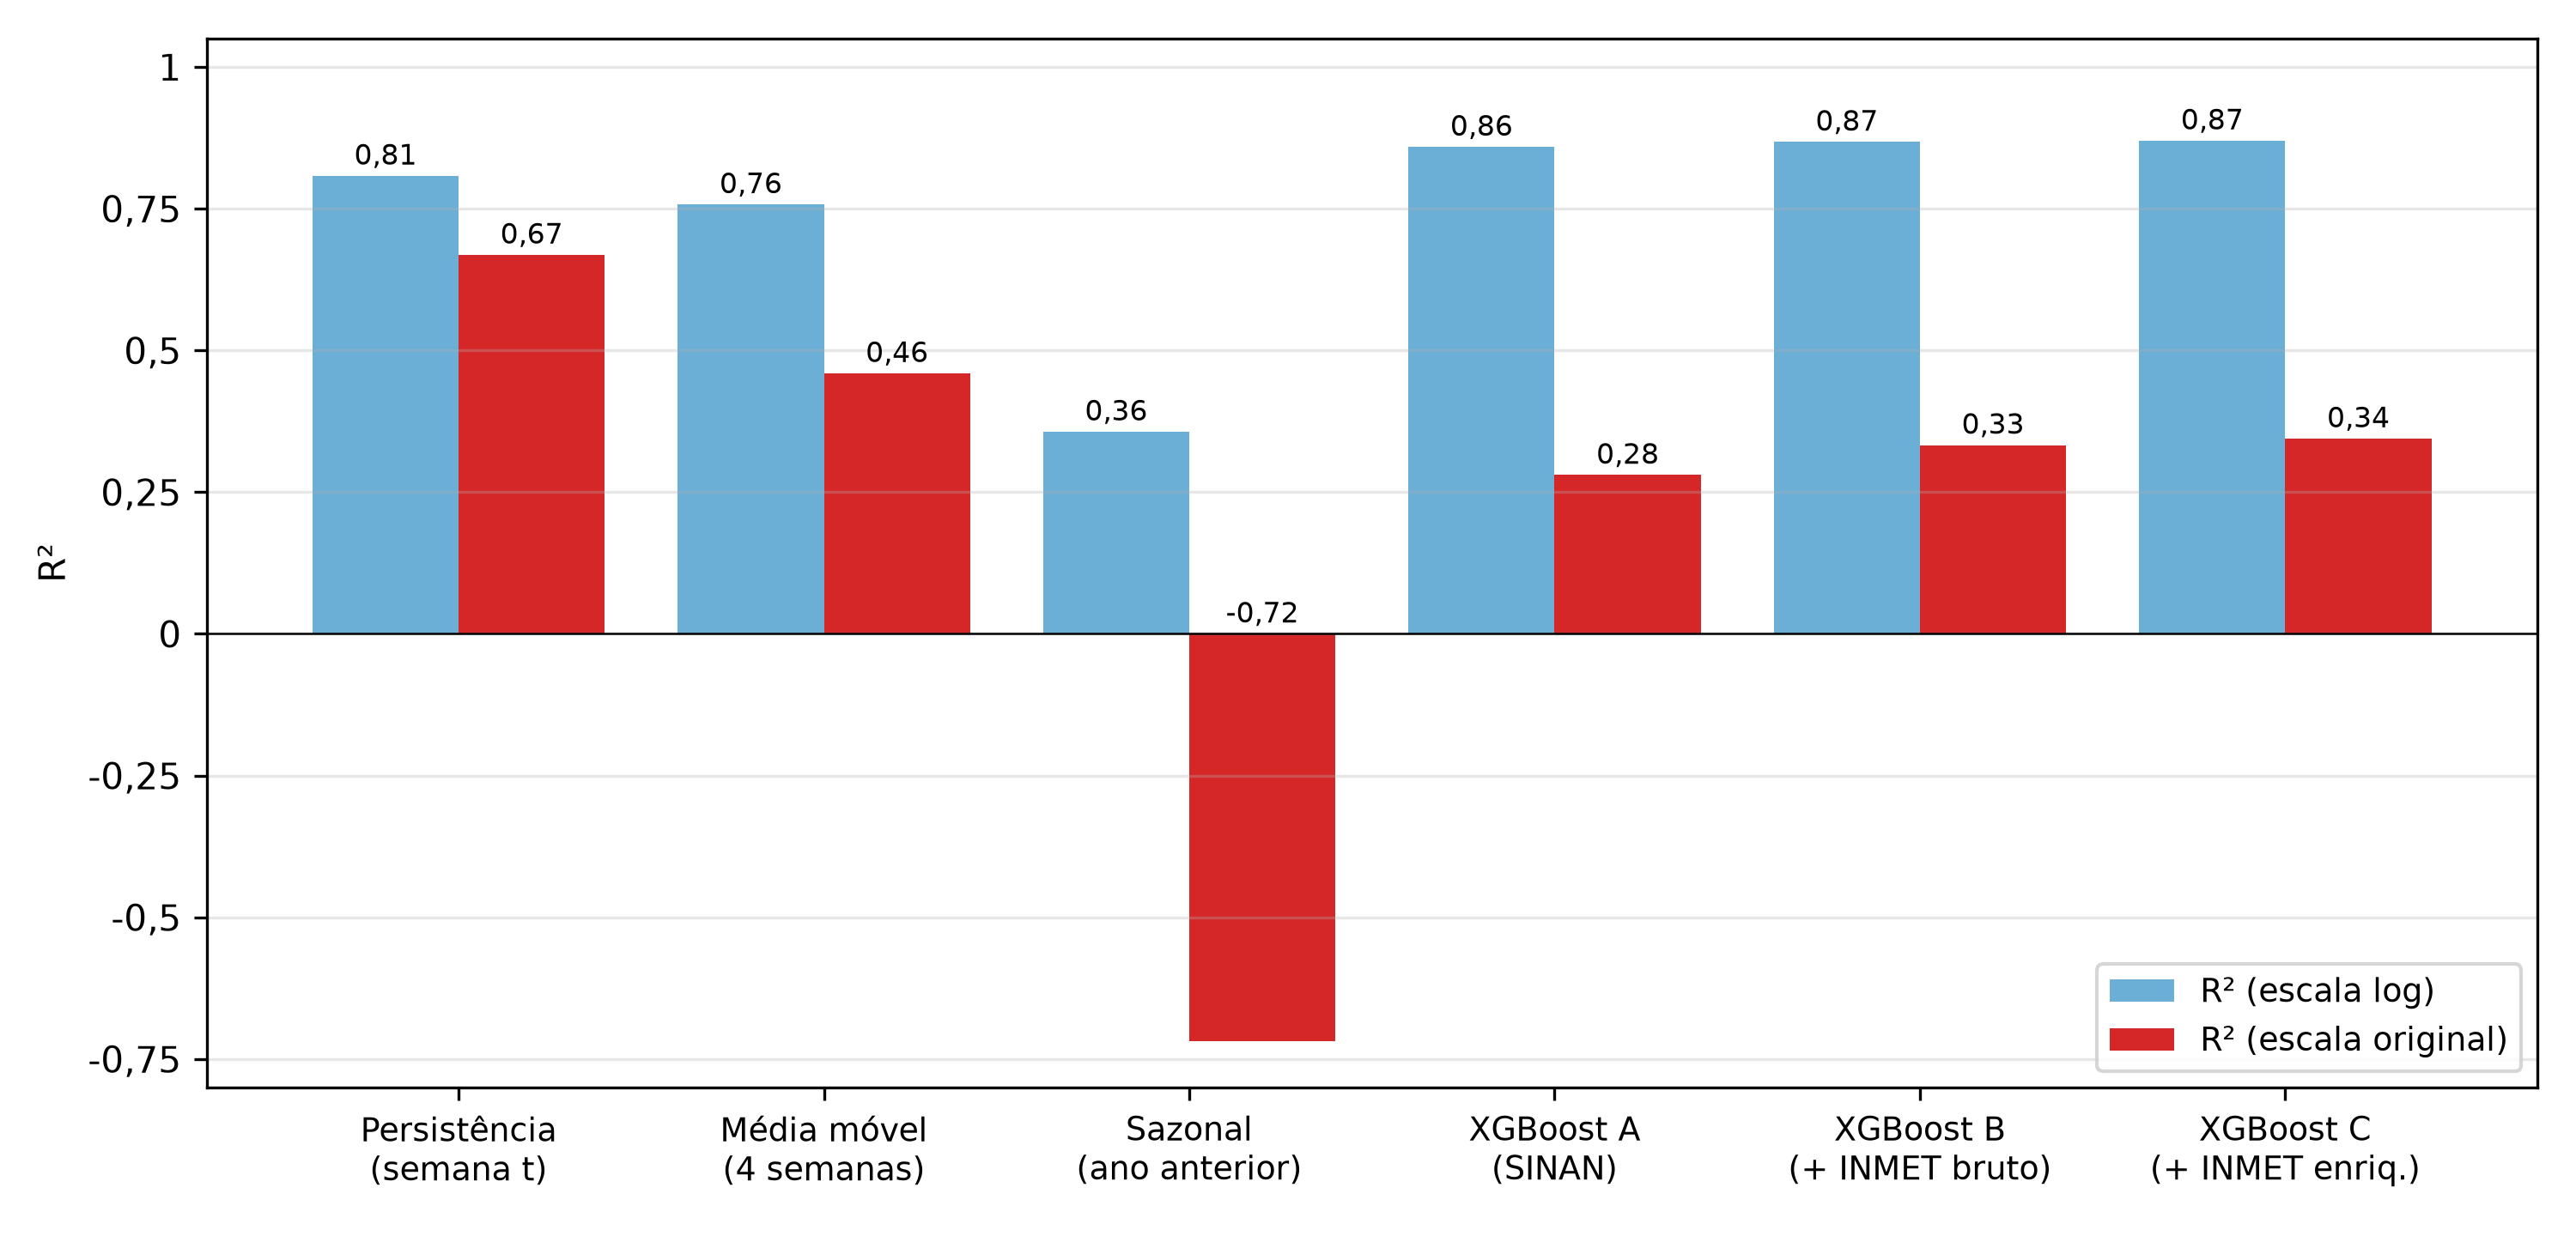
\includegraphics[width=\textwidth]{figuras/resultados/fig_baselines_vs_xgboost.png}
    \label{fig:baselines}
    \fonte{Elaboração própria.}
\end{figure}

As duas escalas medem coisas diferentes (Capítulo~\ref{cap:referencial}). O $R^2_{\log}$ dá peso comparável a todas as mesorregiões e semanas e mostra que o modelo acompanha melhor que os baselines a dinâmica relativa da série, inclusive nas mesorregiões e períodos com poucas notificações. O $R^2$ na escala original é dominado pelas semanas com milhares de notificações, e nelas o modelo erra por muito. O baseline sazonal, com $R^2$ negativo, confirma que repetir o ano anterior é pior que prever a média: a dengue não se repete de um ano para o outro com a mesma intensidade.

\section{Desempenho por Ano e o Evento Epidêmico de 2024}
\label{sec:res_2024}

A desagregação por ano (Tabela~\ref{tab:por_ano}) mostra de onde vem a desvantagem do modelo na escala original. Em 2024, o modelo C previu 3,45 milhões de notificações, quando ocorreram 6,44 milhões; nas 5\% de mesorregião-semanas com mais notificações daquele ano, a previsão cobriu apenas 36\% do total observado, contra 90\% da persistência. Em 2025 e 2026, ao contrário, o modelo C superou a persistência em todas as métricas: $R^2$ de 0,773 contra 0,714 em 2025 e de 0,862 contra 0,763 em 2026, com MAE 29\% e 10\% menor, respectivamente.

\begin{table}[htb]
\centering
\caption{Desempenho por ano de teste: XGBoost e persistência}
\label{tab:por_ano}
\small
\begin{tabular}{|c|l|c|c|r|r|}
\hline
\textbf{Ano} & \textbf{Modelo} & \textbf{$R^2$} & \textbf{$R^2_{\log}$} & \textbf{MAE} & \textbf{Previsto / real (mi)} \\ \hline
2024 & Persistência & \textbf{0,660} & 0,839 & 530,9 & 6,56 / 6,44 \\ \hline
2024 & XGBoost A & 0,247 & 0,889 & 546,6 & 2,89 / 6,44 \\ \hline
2024 & XGBoost C & 0,312 & \textbf{0,903} & \textbf{505,5} & 3,45 / 6,44 \\ \hline
2025 & Persistência & 0,714 & 0,834 & 107,5 & 1,64 / 1,54 \\ \hline
2025 & XGBoost A & 0,692 & 0,885 & 81,2 & 1,21 / 1,54 \\ \hline
2025 & XGBoost C & \textbf{0,773} & \textbf{0,891} & \textbf{76,0} & 1,38 / 1,54 \\ \hline
2026 & Persistência & 0,763 & 0,535 & 56,1 & 0,32 / 0,34 \\ \hline
2026 & XGBoost A & 0,848 & 0,605 & 51,2 & 0,32 / 0,34 \\ \hline
2026 & XGBoost C & \textbf{0,862} & \textbf{0,620} & \textbf{50,5} & 0,33 / 0,34 \\ \hline
\end{tabular}
\fonte{Elaboração própria. Previsto e real em milhões de notificações no ano.}
\end{table}

A Figura~\ref{fig:serie_nacional} mostra o comportamento na série nacional, somando as 137 mesorregiões. Em 2024, o modelo acompanha a subida e a queda da epidemia no tempo certo, mas satura em cerca de metade da altura do pico. A persistência atinge a altura correta, mas com quatro semanas de atraso, que é exatamente o horizonte de previsão. Em 2025 e 2026, o modelo C segue a série observada de perto, enquanto a persistência continua defasada.

\begin{figure}[htb]
    \centering
    \caption{Notificações semanais observadas e previstas no conjunto de teste (soma das 137 mesorregiões)}
    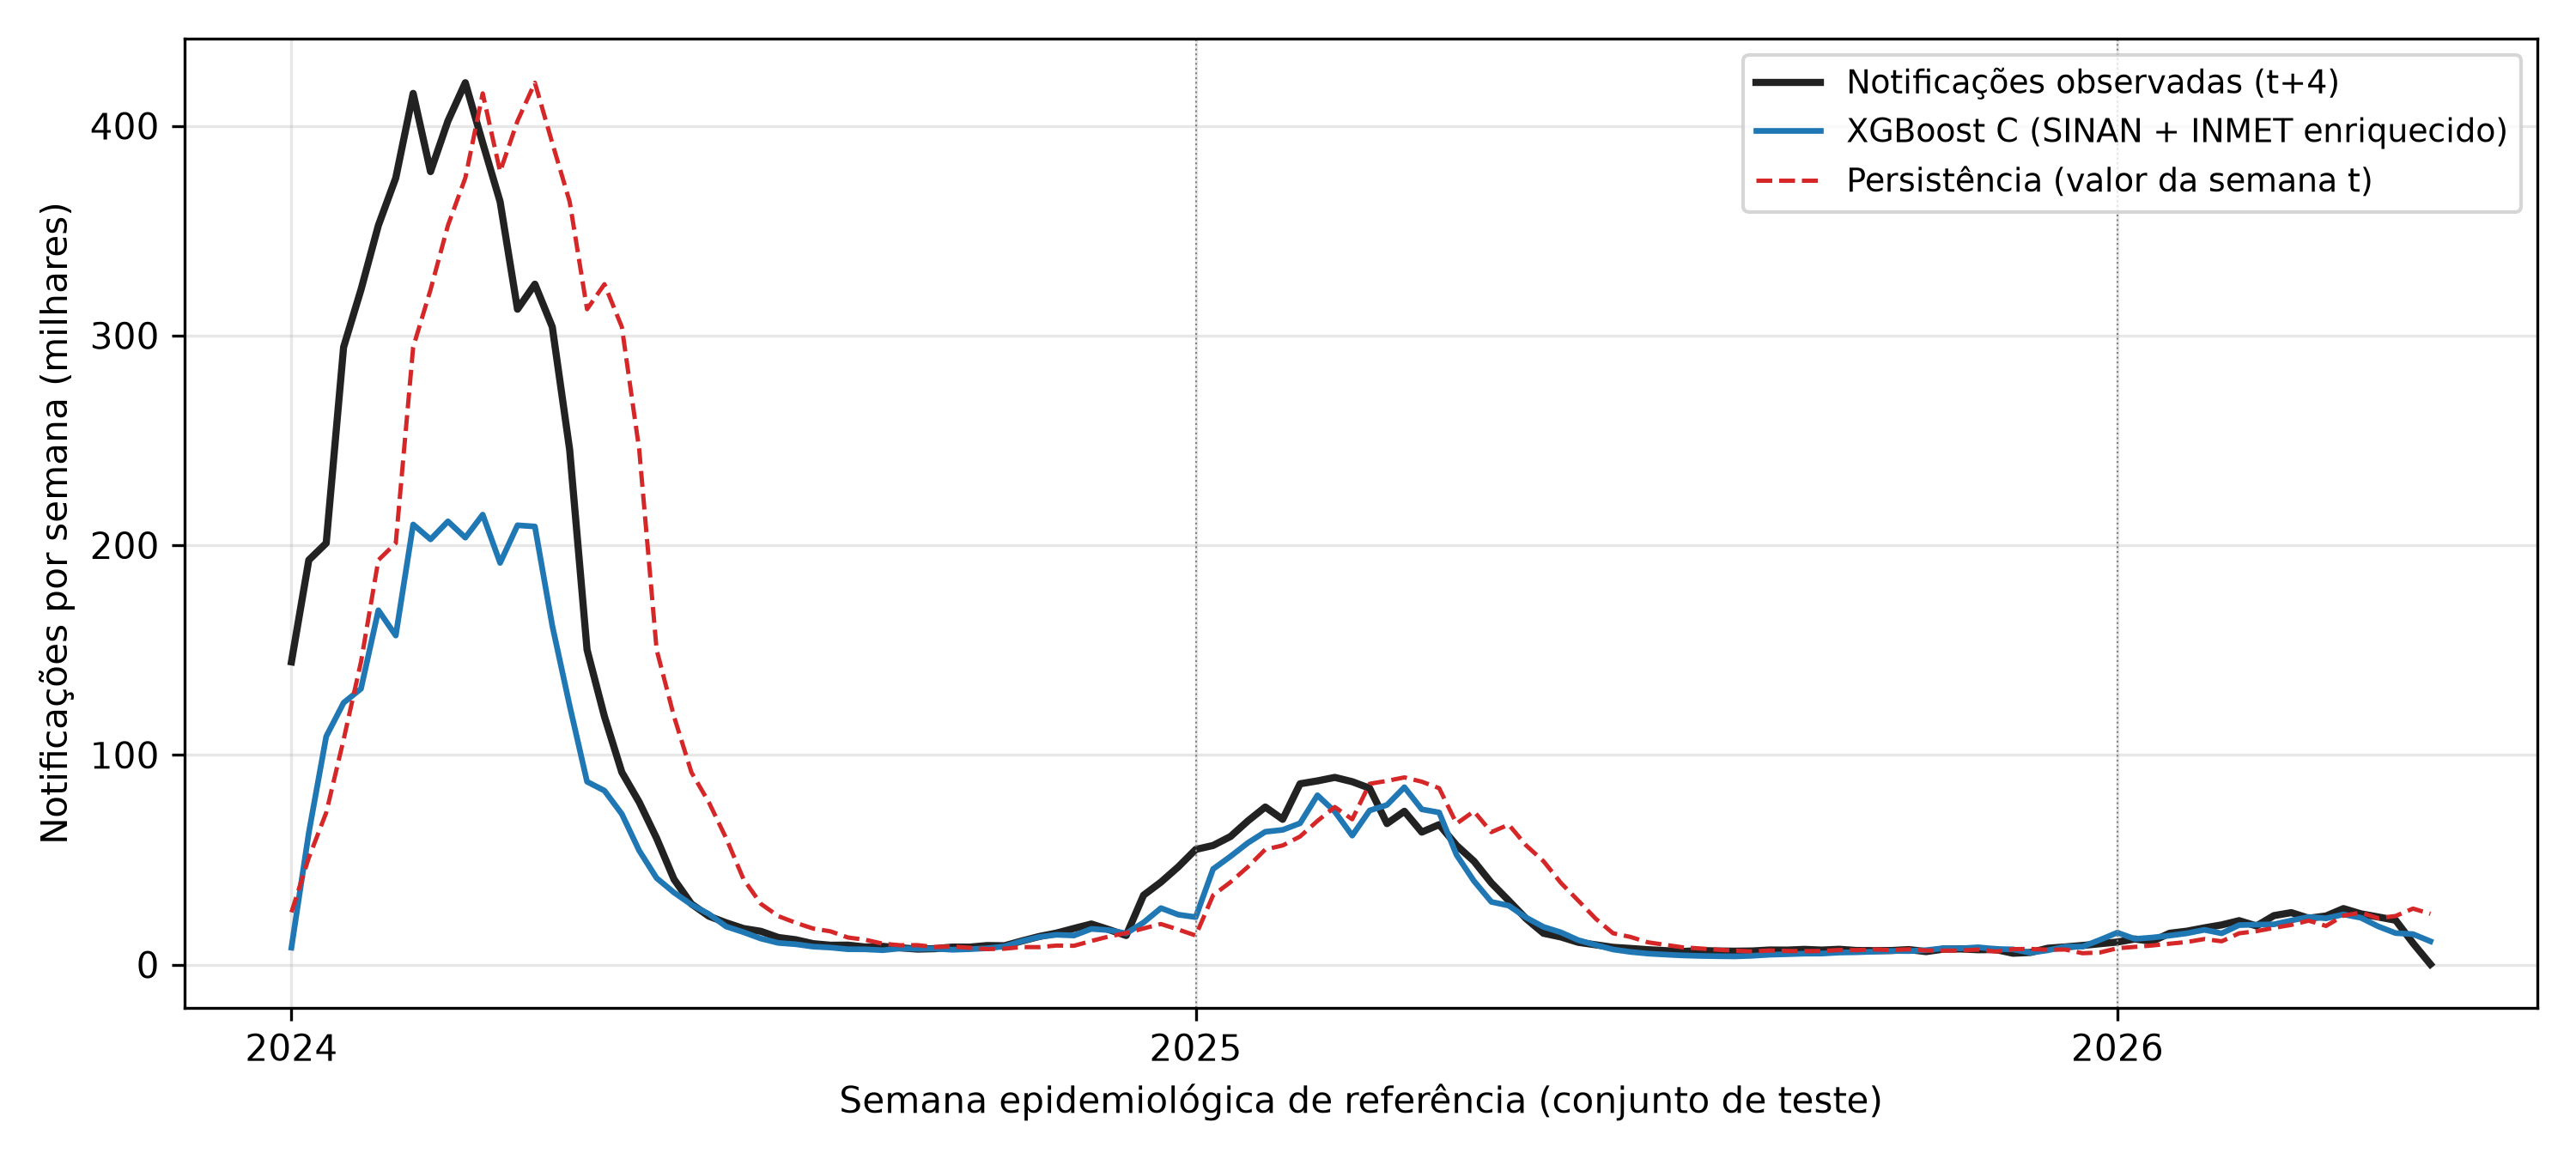
\includegraphics[width=\textwidth]{figuras/resultados/fig_serie_nacional_teste.png}
    \label{fig:serie_nacional}
    \fonte{Elaboração própria.}
\end{figure}

Dois mecanismos, descritos no Capítulo~\ref{cap:referencial}, explicam esse comportamento. O primeiro é a incapacidade de extrapolação das árvores: o maior ano do treino (2019) teve cerca de 2,3 milhões de notificações, e o modelo não consegue produzir valores muito acima da faixa que viu. O segundo é o treinamento sobre $\log(1+y)$, que minimiza erros relativos e tende a subestimar os valores extremos quando a previsão é revertida para a escala original. A persistência, por construção, não tem teto: repete qualquer valor, inclusive um inédito. O resultado responde de forma direta ao ``teste de estresse'' proposto no TCC~1: o modelo antecipa o \textit{momento} de uma epidemia extrema, mas não a sua \textit{magnitude}.

Há ainda um fator de desenho: a contagem de notificações da própria semana $t$, que é exatamente o que a persistência usa, não foi incluída entre os atributos do modelo (a informação mais recente disponível para ele é a contagem de casos confirmados ou prováveis da semana $t$ e as notificações a partir de $t-1$). No experimento complementar, em que essa contagem foi incluída, a diferença para a persistência na escala original foi bem menor ($R^2$ de 0,390 contra 0,400), embora em outro recorte e período de teste (Seção~\ref{sec:res_complementar}).

\section{Contribuição das Variáveis Climáticas}
\label{sec:res_clima}

A inclusão do clima melhorou o modelo de forma pequena, mas consistente e estatisticamente significativa. No teste, o $R^2_{\log}$ passou de 0,859 (A) para 0,868 (B, $\Delta=+0{,}009$, $p<10^{-40}$) e 0,870 (C, $\Delta=+0{,}011$, $p<10^{-30}$); a diferença entre C e B (+0,002, $p<0{,}001$) indica que as defasagens, médias móveis e anomalias acrescentam pouco ao clima da semana corrente. Na escala original, o ganho do clima é maior em termos relativos: o $R^2$ passou de 0,280 para 0,344 e o MAE caiu 7\%.

O ganho se repetiu na validação \textit{walk-forward} (Tabela~\ref{tab:walkforward}): o modelo C superou o A nos quatro anos testados, com média de $R^2_{\log}$ de 0,815 contra 0,799. A tabela também mostra a instabilidade entre anos, com $R^2_{\log}$ entre 0,62 e 0,91: o desempenho depende fortemente das características de cada temporada.

\begin{table}[htb]
\centering
\caption{Validação \textit{walk-forward}: $R^2_{\log}$ por janela (A: só SINAN; B: com clima bruto; C: com clima enriquecido)}
\label{tab:walkforward}
\begin{tabular}{|c|c|c|c|c|}
\hline
\textbf{Treino} & \textbf{Teste} & \textbf{A} & \textbf{B} & \textbf{C} \\ \hline
2019 a 2022 & 2023 & 0,815 & 0,819 & \textbf{0,828} \\ \hline
2019 a 2023 & 2024 & 0,876 & 0,858 & \textbf{0,909} \\ \hline
2019 a 2024 & 2025 & 0,889 & 0,895 & \textbf{0,896} \\ \hline
2019 a 2025 & 2026 & 0,617 & 0,626 & \textbf{0,629} \\ \hline
\multicolumn{2}{|c|}{Média} & 0,799 & 0,799 & \textbf{0,815} \\ \hline
\end{tabular}
\fonte{Elaboração própria.}
\end{table}

Geograficamente, o modelo C superou o A em 22 das 27 UFs e em 103 das 137 mesorregiões. A Figura~\ref{fig:delta_meso} mostra as 20 mesorregiões com maior ganho e as 20 com maior perda: os ganhos chegam a +0,20 de $R^2_{\log}$, e as perdas, principalmente em mesorregiões do Nordeste, a $-$0,14. Essa heterogeneidade é coerente com a literatura, que descreve associações clima--dengue diferentes entre regiões.

\begin{figure}[htb]
    \centering
    \caption{Variação do $R^2_{\log}$ com o clima enriquecido (C $-$ A), por mesorregião (código IBGE): 20 maiores ganhos e 20 maiores perdas}
    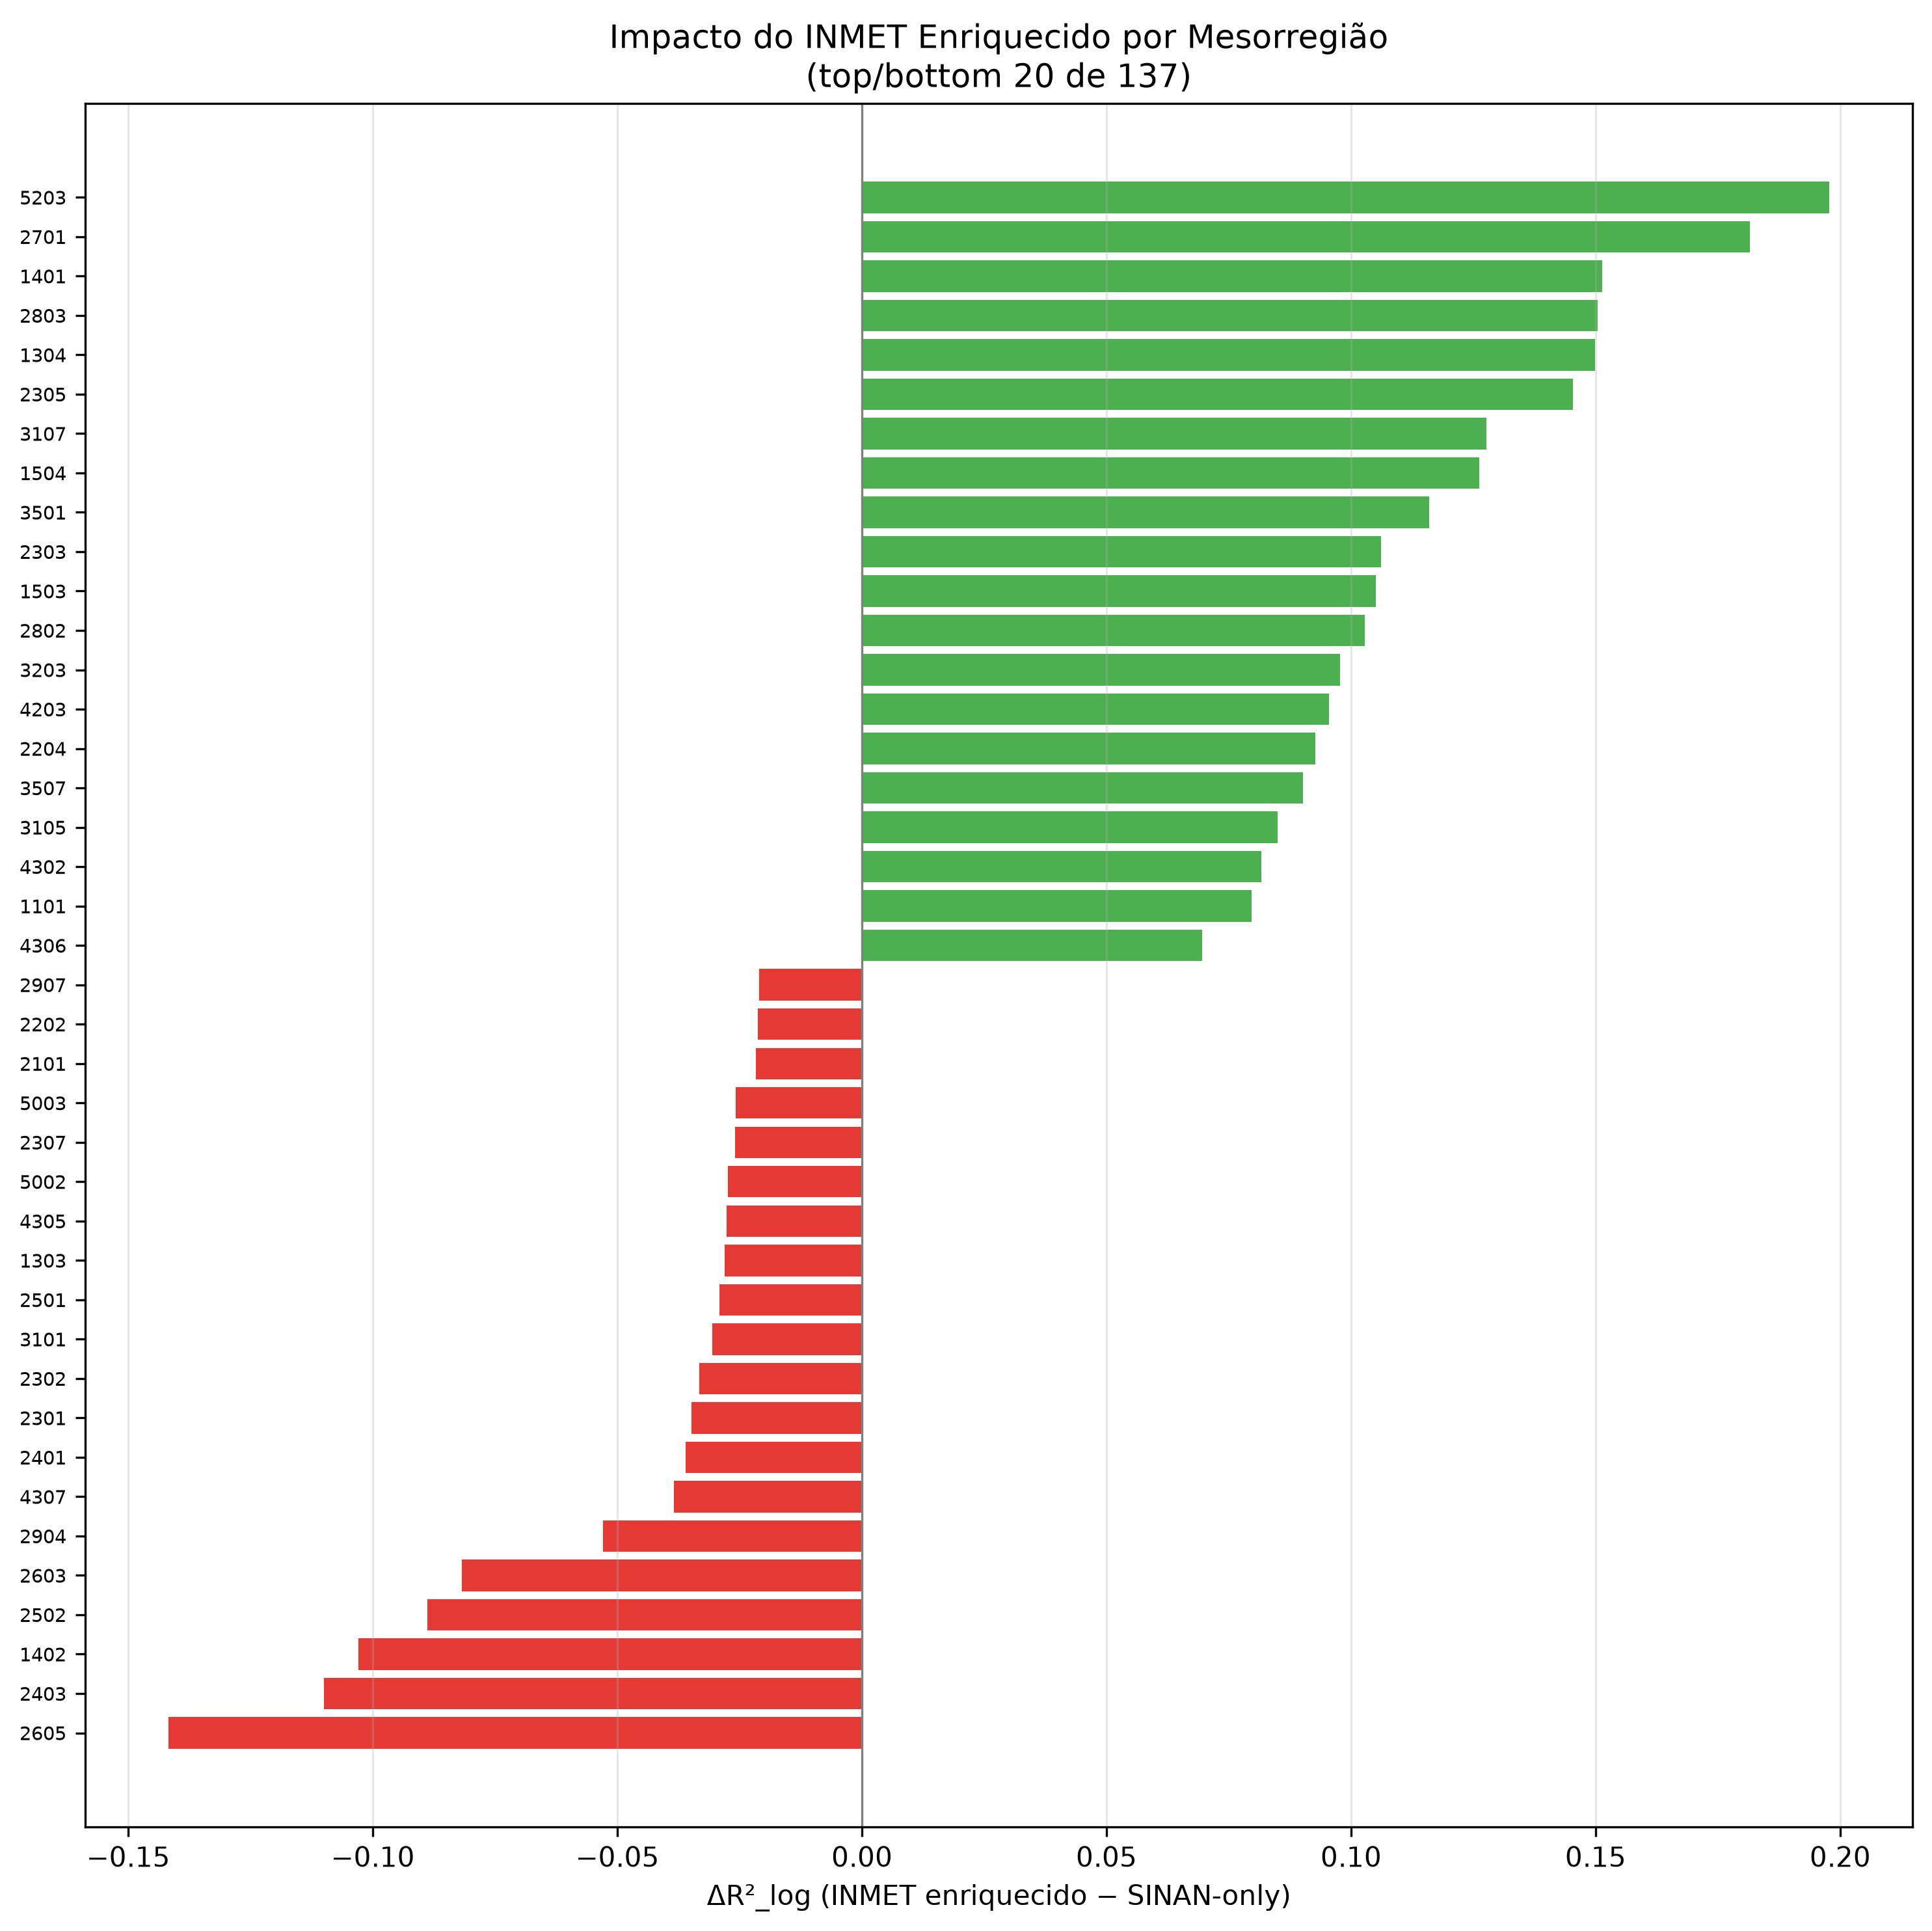
\includegraphics[width=0.75\textwidth]{figuras/resultados/fig_v3_regression_delta_mesorregiao.png}
    \label{fig:delta_meso}
    \fonte{Elaboração própria.}
\end{figure}

\section{Clima na Ausência de Dados Epidemiológicos Recentes}
\label{sec:res_blindness}

A Tabela~\ref{tab:blindness} e a Figura~\ref{fig:blindness} apresentam os cenários de atraso na notificação. Quando as defasagens recentes de notificações são removidas, o clima continua acrescentando informação, e o ganho é significativo com atraso de 4 semanas (+0,0047) e de 8 semanas (+0,0035). No cenário extremo, sem nenhum atributo epidemiológico, o modelo sem clima fica sem nenhuma variável informativa e não tem capacidade preditiva ($R^2_{\log}=-0{,}011$), enquanto as variáveis climáticas sozinhas explicam 39\% da variância em escala logarítmica. Como a codificação da semana do ano também é removida nesse cenário, a sazonalidade que o modelo capta vem apenas do próprio ciclo anual das variáveis climáticas.

\begin{table}[htb]
\centering
\caption{Ganho do clima em cenários de atraso na notificação ($R^2_{\log}$)}
\label{tab:blindness}
\begin{tabular}{|l|c|c|c|c|}
\hline
\textbf{Cenário} & \textbf{Sem clima} & \textbf{Com clima} & \textbf{$\Delta$} & \textbf{$p$} \\ \hline
Completo & 0,859 & 0,870 & +0,011 & $<0{,}001$ \\ \hline
Atraso de 4 semanas & 0,868 & 0,873 & +0,005 & $<0{,}001$ \\ \hline
Atraso de 8 semanas & 0,865 & 0,869 & +0,004 & $<0{,}001$ \\ \hline
Só clima & $-$0,011 & 0,390 & +0,401 & $<0{,}001$ \\ \hline
\end{tabular}
\fonte{Elaboração própria.}
\end{table}

\begin{figure}[htb]
    \centering
    \caption{$R^2_{\log}$ com e sem clima nos cenários de atraso na notificação}
    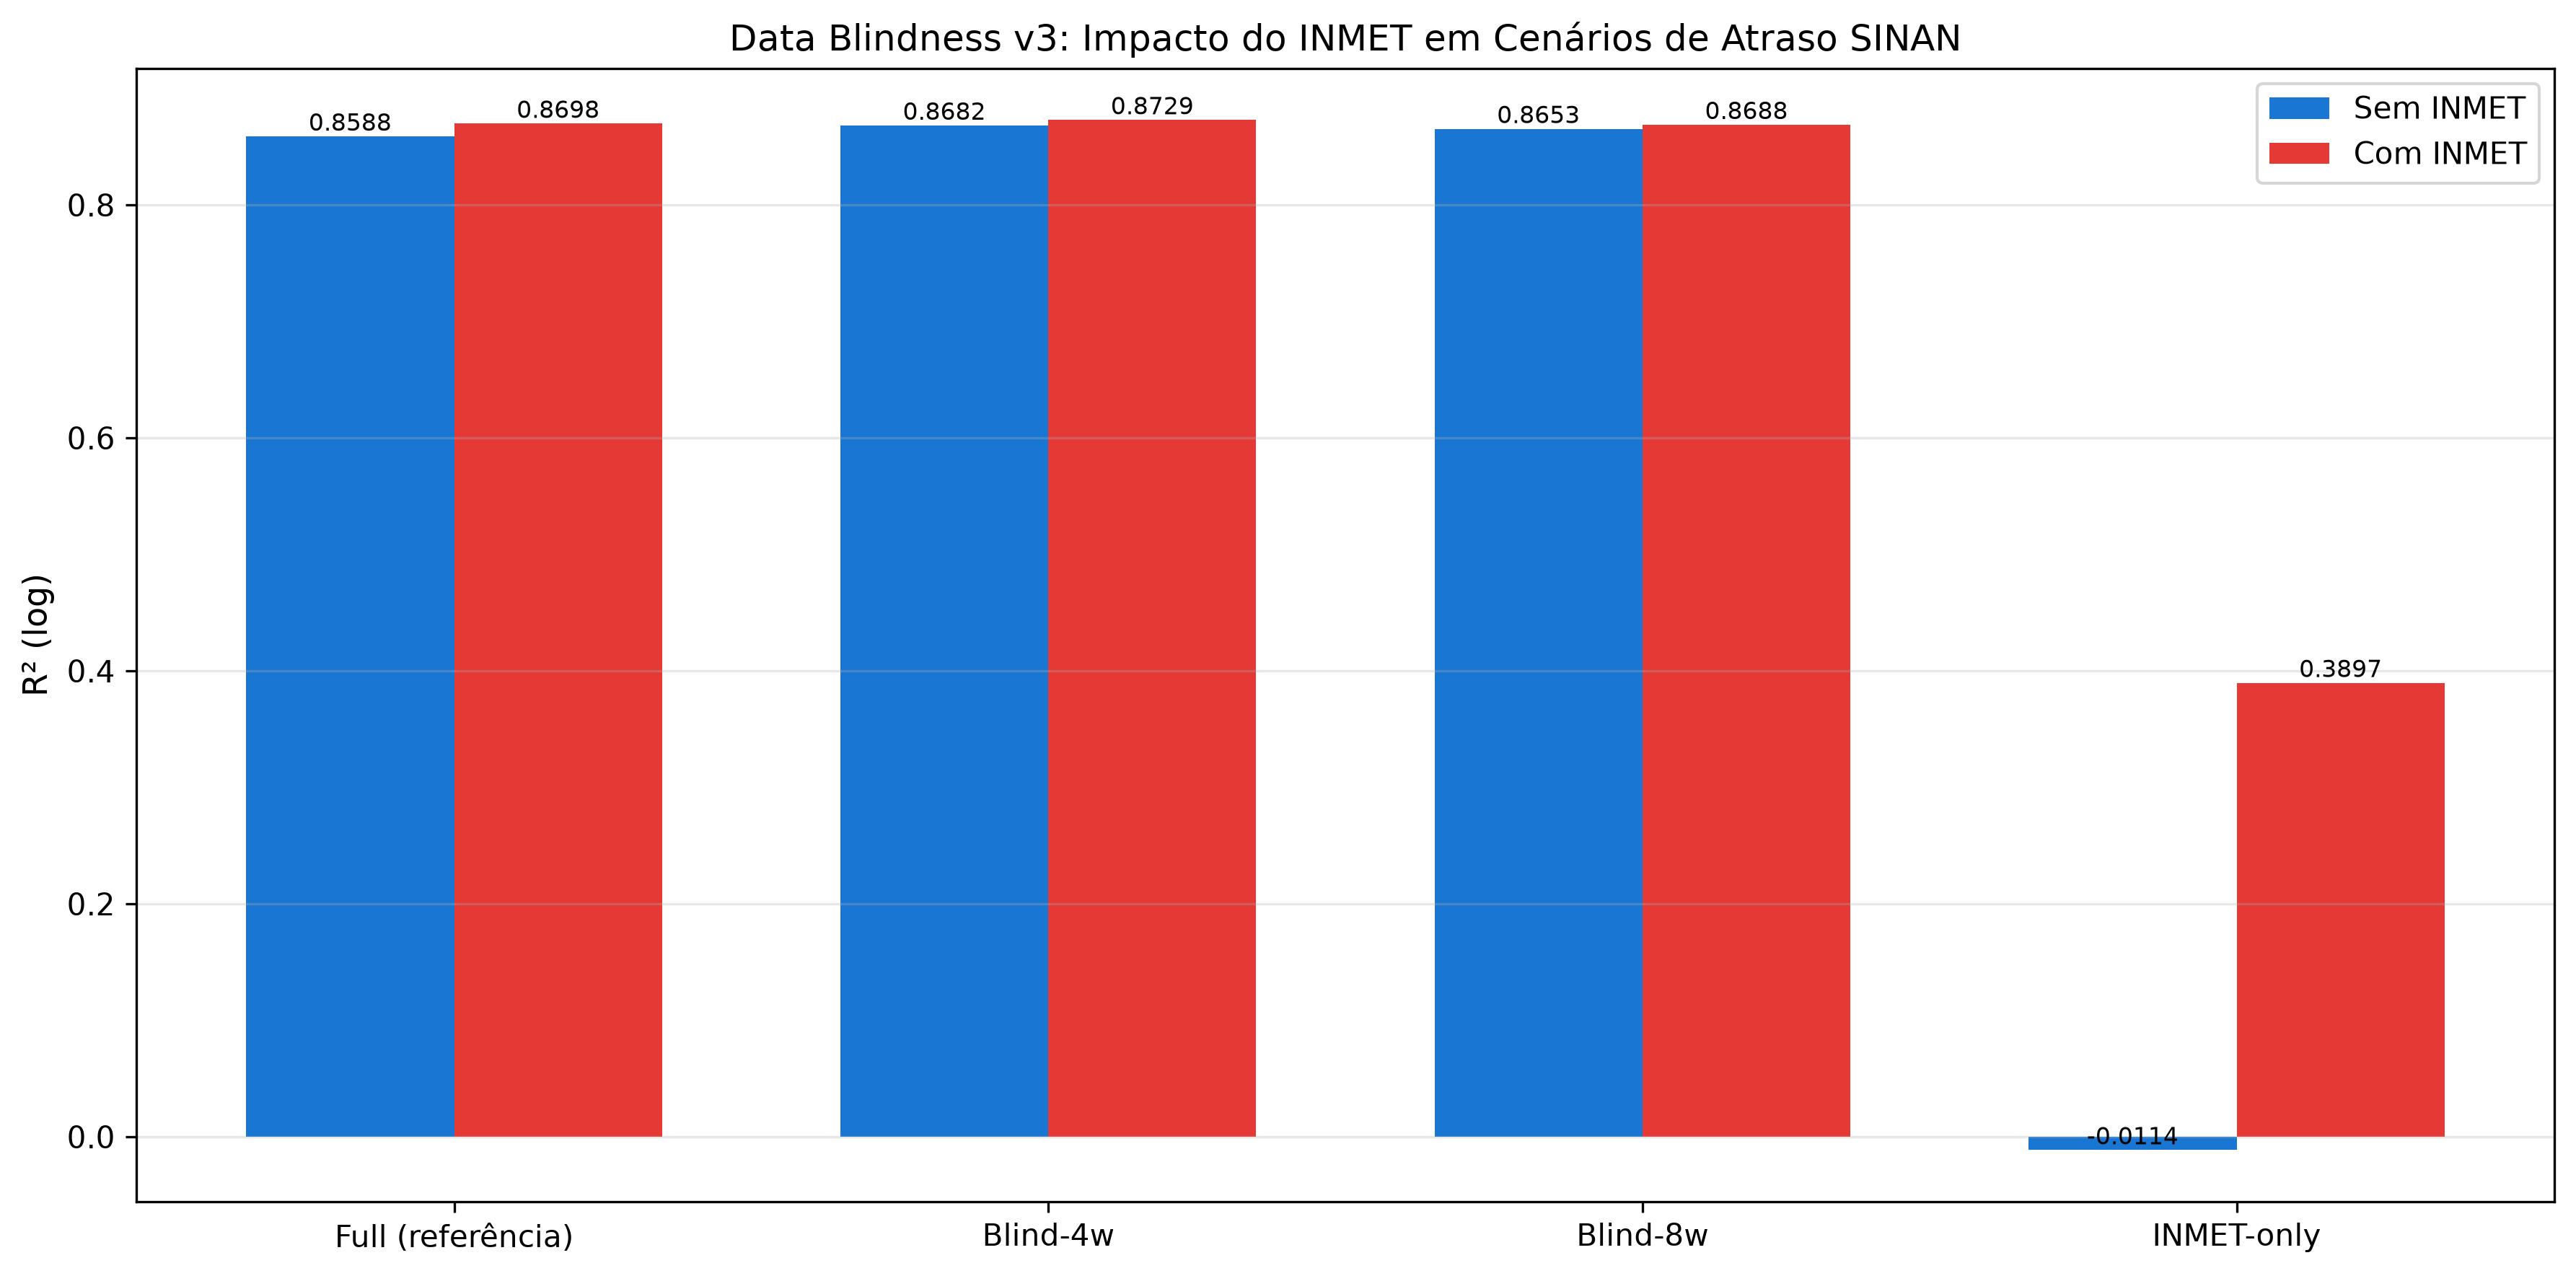
\includegraphics[width=0.9\textwidth]{figuras/resultados/fig_v3_blindness_comparison.png}
    \label{fig:blindness}
    \fonte{Elaboração própria.}
\end{figure}

Esses resultados devem ser lidos com a limitação apontada na metodologia: os cenários de atraso removem as defasagens de notificações, mas mantêm as contagens agregadas da semana $t$, como casos confirmados ou prováveis, o que explica por que o desempenho quase não cai. Uma simulação mais realista do atraso tenderia a reduzir o desempenho sem clima e a aumentar o valor relativo das variáveis climáticas. O cenário ``só clima'' é o limite superior dessa situação e mostra que o clima, sozinho, carrega sinal sobre a dengue quatro semanas à frente, embora bem inferior ao da série epidemiológica.

\section{Interpretação do Modelo}
\label{sec:res_shap}

A análise SHAP do modelo C (Figura~\ref{fig:shap}) mostra que a previsão é dominada pela própria série epidemiológica: as notificações da semana anterior respondem sozinhas por uma contribuição média (0,91) mais de três vezes maior que a segunda variável, a contagem de casos confirmados ou prováveis (0,25). A codificação da semana do ano ocupa a 3.ª e a 6.ª posições, refletindo a sazonalidade. Nenhuma variável climática aparece entre as dez mais importantes; a primeira é a temperatura mínima da semana, na 20.ª posição, e nove variáveis climáticas aparecem entre as 30 primeiras. A contribuição média das variáveis climáticas foi cerca de cinco vezes menor que a das epidemiológicas (0,004 contra 0,021).

\begin{figure}[htb]
    \centering
    \caption{Valores SHAP das 20 variáveis mais importantes do modelo C}
    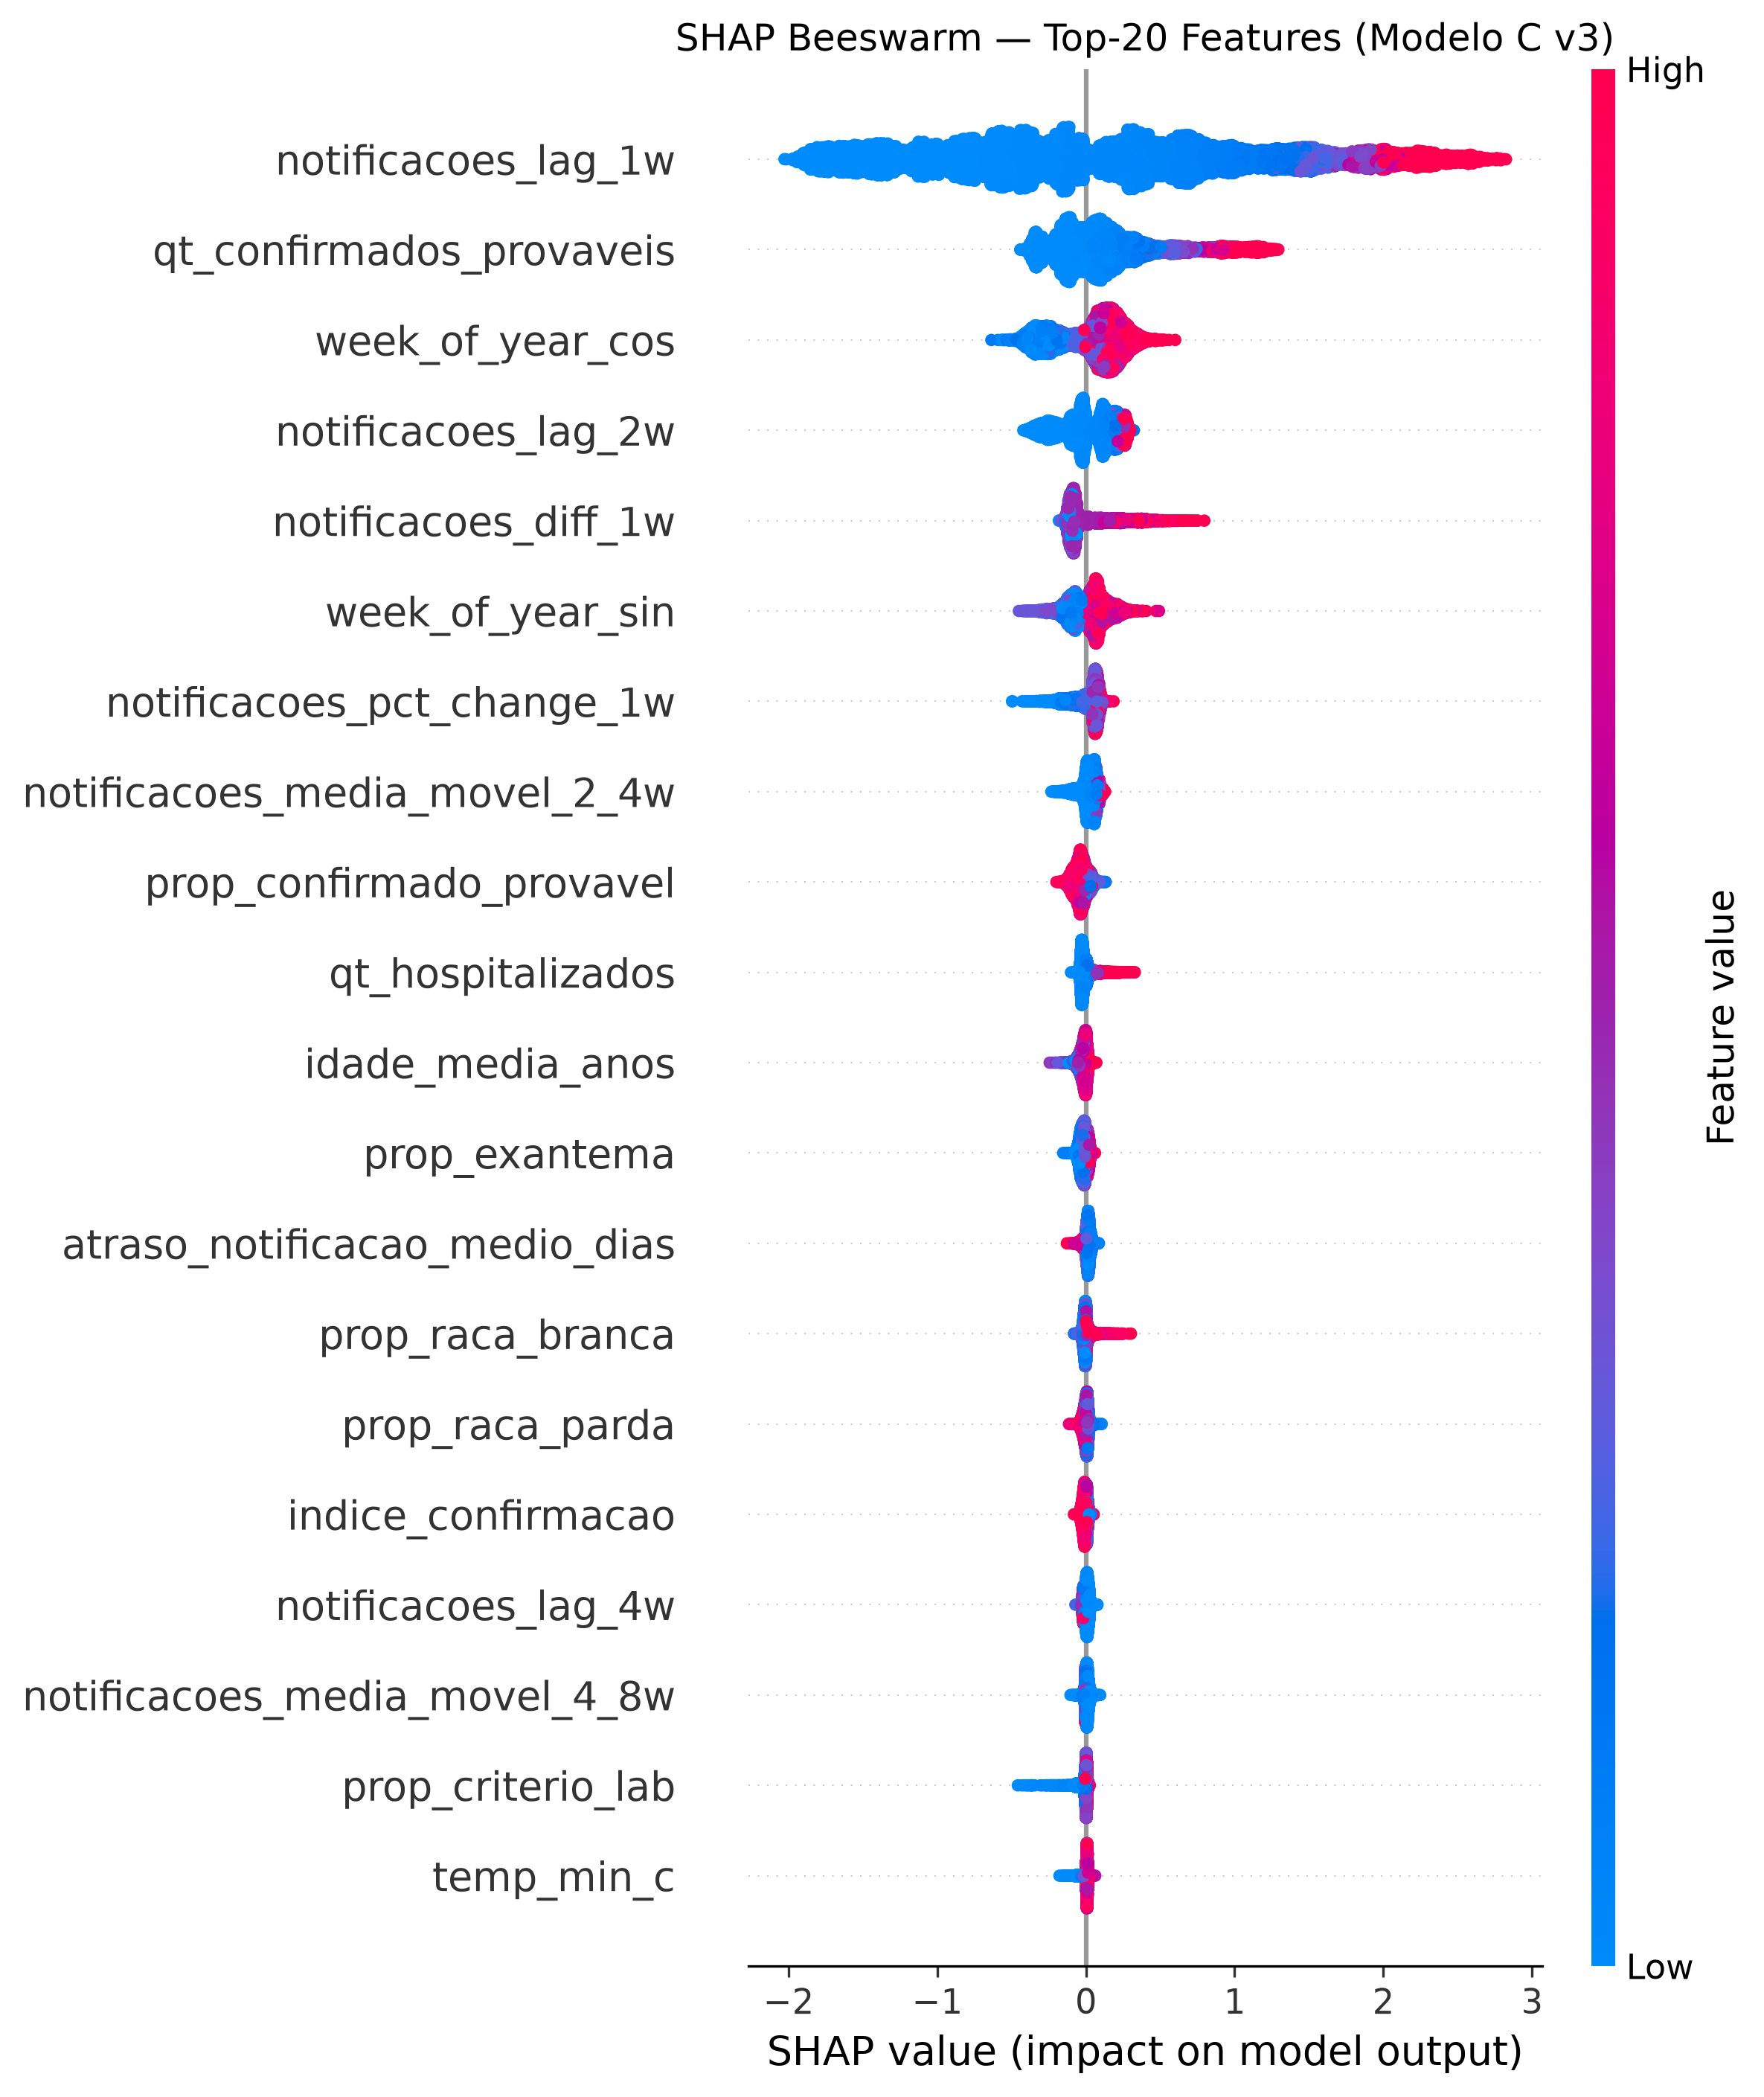
\includegraphics[width=0.7\textwidth]{figuras/resultados/fig_v3_shap_beeswarm.png}
    \label{fig:shap}
    \fonte{Elaboração própria.}
\end{figure}

Os limiares estimados para as variáveis climáticas (Tabela~\ref{tab:limiares}) são coerentes com a biologia do vetor. A contribuição da temperatura passa a ser positiva acima de 13,8~$^\circ$C de mínima e de 21,0~$^\circ$C de média semanal, valores próximos do limite inferior de transmissão descrito na literatura. A precipitação média na janela de 2 a 4 semanas e o número de dias de chuva nessa janela aumentam a previsão, o que corresponde ao intervalo de desenvolvimento do vetor. A pressão atmosférica tem efeito negativo, provavelmente como indicador indireto de altitude e de massas de ar mais secas e frias.

\begin{table}[htb]
\centering
\caption{Limiares climáticos estimados pela análise SHAP (modelo C) e efeito sobre a previsão acima do limiar}
\label{tab:limiares}
\small
\begin{tabular}{|p{0.47\textwidth}|c|r|c|}
\hline
\textbf{Variável} & \textbf{Posição} & \textbf{Limiar} & \textbf{Efeito} \\ \hline
Temperatura mínima (semana $t$) & 20 & 13,8~$^\circ$C & aumenta \\ \hline
Temperatura média (semana $t$) & 21 & 21,0~$^\circ$C & aumenta \\ \hline
Precipitação média, média de 2 a 4 semanas & 22 & 0,11~mm/h & aumenta \\ \hline
Radiação média, média de 4 a 8 semanas & 23 & 1.317~kJ/m$^2$ & aumenta \\ \hline
Pressão média, 8 semanas antes & 25 & 992~hPa & reduz \\ \hline
Pressão média, média de 4 a 8 semanas & 27 & 981~hPa & reduz \\ \hline
Dias de chuva, média de 2 a 4 semanas & 28 & 2,1 dias & aumenta \\ \hline
Precipitação acumulada, média de 2 a 4 semanas & 29 & 16,1~mm & aumenta \\ \hline
Temperatura mínima, média de 2 a 4 semanas & 30 & 15,3~$^\circ$C & aumenta \\ \hline
\end{tabular}
\fonte{Elaboração própria.}
\end{table}

\section{Classificação do Nível de Risco}
\label{sec:res_risco}

Na classificação em quatro níveis de risco (Tabela~\ref{tab:risco}), o XGBoost dedicado alcançou F1 macro de 0,49 e AUC de 0,77 com clima, contra 0,47 e 0,75 sem clima. Todos os classificadores, no entanto, ficaram abaixo da simples aplicação dos limiares de risco à persistência, que obteve F1 macro de 0,62 e foi superior em todas as classes. As classes intermediárias (moderado e alto) foram as mais difíceis para todos os métodos.

\begin{table}[htb]
\centering
\caption{Classificação do nível de risco no conjunto de teste (F1)}
\label{tab:risco}
\small
\begin{tabular}{|l|c|c|c|c|c|}
\hline
\textbf{Modelo} & \textbf{Macro} & \textbf{Baixo} & \textbf{Moderado} & \textbf{Alto} & \textbf{Muito alto} \\ \hline
Persistência & \textbf{0,622} & \textbf{0,837} & \textbf{0,481} & \textbf{0,416} & \textbf{0,755} \\ \hline
Média móvel (4 semanas) & 0,578 & 0,810 & 0,431 & 0,372 & 0,700 \\ \hline
XGBoost A (só SINAN) & 0,470 & 0,724 & 0,286 & 0,263 & 0,609 \\ \hline
XGBoost B (+ INMET bruto) & 0,491 & 0,740 & 0,323 & 0,268 & 0,632 \\ \hline
XGBoost C (+ INMET enriquecido) & 0,491 & 0,736 & 0,299 & 0,284 & 0,643 \\ \hline
\end{tabular}
\fonte{Elaboração própria.}
\end{table}

O experimento complementar chegou ao mesmo resultado com uma definição de surto diferente, binária e baseada no canal endêmico: o classificador dedicado obteve F1 de 0,72 a 0,74 para a classe surto, abaixo da persistência do rótulo (0,85). Aplicar o limiar do canal endêmico à previsão contínua da regressão, em vez de treinar um classificador, alcançou 0,83, próximo à persistência. Os dois resultados indicam que, para gerar alertas, é preferível derivá-los da previsão numérica, e não treinar um classificador separado.

\section{Recorte do Distrito Federal}
\label{sec:res_df}

O Distrito Federal, foco do TCC~1, corresponde a uma única mesorregião, com 124 semanas no teste. Nele, o clima trouxe o maior ganho entre as 27 UFs: o $R^2_{\log}$ passou de 0,722 (A) para 0,789 (C) e o $R^2$ na escala original de 0,333 para 0,466. Ainda assim, a persistência foi superior ($R^2_{\log}=0{,}826$ e $R^2=0{,}647$). O padrão é o mesmo do agregado nacional: o modelo subestimou o total do período, prevendo cerca de 155 mil notificações para 256 mil observadas, principalmente pela epidemia de 2024.

\section{Verificação Independente: Experimento Complementar}
\label{sec:res_complementar}

O experimento complementar, com dados de outro recorte (seis UFs), outra divisão temporal (teste em 2023) e a contagem da semana $t$ incluída nos atributos, confirmou os achados principais (Tabela~\ref{tab:complementar}). Em nível municipal, o XGBoost superou a persistência em $R^2_{\log}$ e MAE, mas não em $R^2$ na escala original; o clima acrescentou +0,029 de $R^2$. Agregado por mesorregião, o modelo com clima superou a persistência também na escala original (0,487 contra 0,397), e o ganho do clima foi o maior observado (+0,106). No nível de UF, com apenas seis séries, o clima não ajudou.

\begin{table}[htb]
\centering
\caption{Experimento complementar (seis UFs, teste em 2023): $R^2$ na escala original da persistência e do XGBoost com e sem clima}
\label{tab:complementar}
\small
\begin{tabular}{|l|c|c|c|c|}
\hline
\textbf{Agregação} & \textbf{Persistência} & \textbf{Só SINAN} & \textbf{SINAN + INMET} & \textbf{Ganho do clima} \\ \hline
Município & \textbf{0,400} & 0,361 & 0,390 & +0,029 \\ \hline
Mesorregião & 0,397 & 0,381 & \textbf{0,487} & +0,106 \\ \hline
UF & 0,454 & \textbf{0,625} & 0,528 & $-$0,097 \\ \hline
\end{tabular}
\fonte{Elaboração própria a partir de \citeonline{modeloprevisao2026}.}
\end{table}

\section{Síntese}

Os resultados respondem às três questões operacionais formuladas na introdução:

\begin{enumerate}
    \item \textbf{XGBoost contra baselines.} O XGBoost supera os previsores ingênuos em escala logarítmica e em erro absoluto, e supera a persistência em todas as métricas nos anos típicos (2025 e 2026). No evento extremo de 2024, antecipa o momento da epidemia, mas subestima a sua magnitude em cerca de metade, e perde para a persistência na escala original. Para classificar o nível de risco, a persistência é superior a um classificador dedicado.
    \item \textbf{Contribuição do clima.} O ganho é pequeno em relação à informação epidemiológica, mas consistente: significativo no teste, presente em todas as janelas do \textit{walk-forward}, em 22 das 27 UFs e em 103 das 137 mesorregiões, e mantido quando os dados epidemiológicos recentes estão ausentes. Sem nenhuma informação epidemiológica, o clima sozinho explica 39\% da variância em escala logarítmica.
    \item \textbf{Variáveis e limiares.} A temperatura (mínima acima de 13,8~$^\circ$C e média acima de 21~$^\circ$C) e a chuva na janela de 2 a 4 semanas são as variáveis climáticas mais utilizadas, com limiares coerentes com a biologia do vetor. A associação com a ``umidade'' encontrada em versões anteriores era um artefato de dados.
\end{enumerate}
